% 3. Methods [title could be made less generic]
% - [Describe and argue for own methodology/approach: how does your approach work, why did you choose it? The latter could also be discussed in ch. 2]



\section{Overview}

Our experimental framework utilizes the \gls{ssast} model developed by \cite{gong2022ssast}. The architecture of this model is depicted in Figure \ref{fig:ssast_architecture}.

\begin{figure}[h]
    \centering
    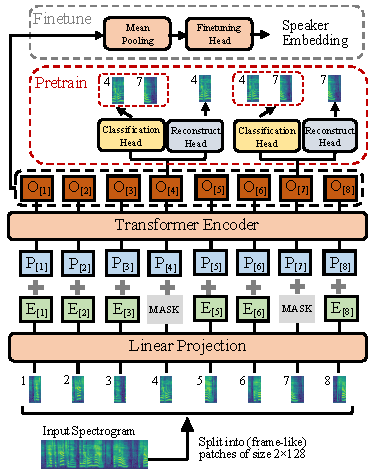
\includegraphics[width=0.6\linewidth]{img/ssast_architecture_frame.pdf}
    \caption{Architecture of the (frame-based) SSAST (adapted from \cite{gong2022ssast}).}
    \label{fig:ssast_architecture}
\end{figure}

To assess the impact of temporal structure in audio spectrograms for \gls{sv} tasks, we compare the performance of models trained on unaltered spectrograms with those trained on temporally shuffled spectrograms.

\section{Data}
\label{methods_datasets}

\subsection{Conversion to Mel Spectrogram}
\label{sec:mel_spectrogram_conversion}

Given a discrete audio waveform ${s} \in \mathbb{R}^l$ sampled at a sampling frequency $f_s$, where ${s}[n]$ denotes the $n$-th sample in the audio signal and $l$ is the number of samples in the audio signal, the Mel spectrogram can be computed\footnote{See \href{https://pytorch.org/audio/main/\_modules/torchaudio/compliance/kaldi.html\#fbank}{https://pytorch.org/audio/main/\_modules/torchaudio/compliance/kaldi.html\#fbank} for more details.} as described in the following paragraphs \cite{yang2021torchaudio, hwang2023torchaudio}. Figure \ref{fig:main_steps_signal_into_melspectrogram} illustrates the main steps of the conversion on a high level.

\begin{figure}[h]

    \centering
    
    \begin{tikzpicture}[
            font=\footnotesize, 
            %thick, 
            node distance=0.45cm, 
            auto 
        ]
        
        % Define styles
        \tikzstyle{block} = [rectangle, draw, text width=4.6em, text centered, minimum height=3.5em]
        \tikzstyle{line} = [draw, -Latex]

    
         % Nodes
         
        \node (acoustic) {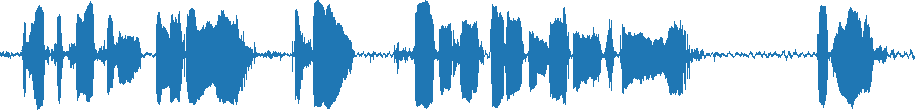
\includegraphics[scale=0.9, clip, viewport=0 0 0.166\imagewidth{} 0.93\imageheight{}]{img/waveform.pdf}};
        
        \node[block, right=0.7cm of acoustic] (windowing) {
            \begin{tikzpicture}[yscale=1, xscale=0.8]
                \draw[smooth, domain=-1:1, samples=20, variable=\x] plot ({\x}, {0.5*(cos(deg(0.5*pi*\x)))^2});
            \end{tikzpicture}
        };

        \node[block, right=0.8cm of windowing] (fourier) {$t \xrightarrow{\text{\Large$\mathscr{F}$}} f$};
        
        % \node[block, right=0.8cm of fourier] (melbank) {};
        % % mel fbanks
        % \setlength{\melwidth}{4.2em} 
        % \setlength{\melheight}{1em}
        % \draw ([shift={(0.0\melwidth, 0.0\melheight)}]melbank.south west) -- ([shift={(0.064\melwidth, 1.0\melheight)}]melbank.south west) -- ([shift={(0.145\melwidth, 0.0\melheight)}]melbank.south west);
        \node[block, right=0.8cm of fourier] (melbank) {
            \begin{tikzpicture}
                \setlength{\melwidth}{5.4em} 
                \setlength{\melheight}{2.3em}
                \draw[red!60!black] (0.0\melwidth, 0.0\melheight) -- (0.064\melwidth, 1.0\melheight) -- (0.145\melwidth, 0.0\melheight);
                \draw[red!80!black] (0.064\melwidth, 0.0\melheight) -- (0.145\melwidth, 1.0\melheight) -- (0.246\melwidth, 0.0\melheight);
                \draw[red] (0.145\melwidth, 0.0\melheight) -- (0.246\melwidth, 1.0\melheight) -- (0.375\melwidth, 0.0\melheight);
                \draw[orange!20!red] (0.246\melwidth, 0.0\melheight) -- (0.375\melwidth, 1.0\melheight) -- (0.537\melwidth, 0.0\melheight);
                \draw[orange!60!red] (0.375\melwidth, 0.0\melheight) -- (0.537\melwidth, 1.0\melheight) -- (0.741\melwidth, 0.0\melheight);
                \draw[orange] (0.537\melwidth, 0.0\melheight) -- (0.741\melwidth, 1.0\melheight) -- (1.0\melwidth, 0.0\melheight);
            \end{tikzpicture}
        };

        \node[right=0.7cm of melbank] (melspec) {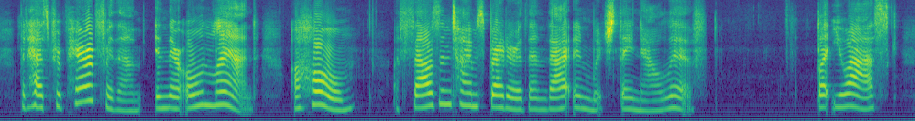
\includegraphics[scale=0.8, clip, viewport=0 0 0.168\imagewidth{} 1.0\imageheight{}]{img/spectrogram.pdf}};

        % Arrows
        \draw[line] (acoustic) -- ($(windowing.west) - (0.3em, 0)$);
        \draw[line] ($(windowing.east) + (0.3em, 0)$) -- ($(fourier.west) - (0.3em, 0)$);
        \draw[line] ($(fourier.east) + (0.3em, 0)$) -- ($(melbank.west) - (0.3em, 0)$);
        \draw[line] ($(melbank.east) + (0.3em, 0)$) -- (melspec);

                % Labels
        \coordinate (LabelBase) at ([yshift=0.4em]acoustic.north);
        \node[anchor=base] at (LabelBase -| acoustic) {Raw Waveform};
        \node[anchor=base] at (LabelBase -| windowing) {Windowing};
        \node[anchor=base] at (LabelBase -| fourier) {Fourier Transform};
        \node[anchor=base] at (LabelBase -| melbank) {Mel Filters};
        \node[anchor=base] at (LabelBase -| melspec) {Mel Spectrogram};
        
    \end{tikzpicture}

    \caption{Main steps for converting an acoustic signal into a Mel spectrogram.}
    \label{fig:main_steps_signal_into_melspectrogram}
\end{figure}


\subsubsection{Windowing and Frame Striding}
The signal \({s}\) is divided into overlapping frames using a stride of \(S\) and a window length of \(W\). This results in \(L\) frames where 
\begin{equation}
\label{eq:spectrogram_L}   
L = \left\lfloor \frac{l - W}{S} + 1 \right\rfloor.
\end{equation}
The floor function, denoted by \(\lfloor \cdot \rfloor\), ensures that only complete frames are used. Each frame \({s}_i\), where \(i \in \{0, 1, \ldots, L-1\}\), is centered as follows:
\begin{equation}
\label{eq:timedomain_frames}
{s}_i = ({s}[h : h+W-1] - \mu_{{s}_i}), \quad \text{for } h = i \cdot S,
\end{equation}
where \(\mu_{{s}_i}\) is the mean of the frame.

\subsubsection{Pre-emphasis Filtering}
After centering, a pre-emphasis filter is applied to each frame to accentuate higher frequencies:
\begin{equation}
\label{eq:preemphasis}
{s}_i'[n] = {s}_i[n] - \alpha \cdot {s}_i[n-1]
\end{equation}
where \(\alpha = 0.97\) is the pre-emphasis coefficient.

\subsubsection{Window Function}
To minimize spectral leakage, each frame \({s}_i'\) is then multiplied element-wise with a window:
\begin{equation}
{s}_i'' = {s}_i' \odot {w}
\end{equation}
where \({w}\) is obtained using a windowing function (e.g. Hanning).


\subsubsection{Fourier Transform and Power Spectrum}
Each frame is zero-padded to the nearest power of two, \(W_{\text{pad}}\), and transformed into the frequency domain using the \gls{fft} \cite{Cooley1965}. The power spectrum \({P}_i\) of each frame is computed as:
\begin{equation}
\label{eq:power_spectrum} 
{P}_i = \left| \mathscr{F}({s}_i'') \right|^2 \in \mathbb{R}^{\frac{W_{\text{pad}}}{2}+1}
\end{equation}
where \(\mathscr{F}\) denotes the \gls{fft} for a real-valued input signal. These power spectra are then concatenated as columns to create ${P}$, a matrix of size $\left( \frac{W_{\text{pad}}}{2}+1 \right) \times L$.

\subsubsection{Mel Filter Banks}
The Mel scale filter banks are applied to the power spectrum to extract frequency bands that correspond to human auditory perception. This is achieved by mapping frequencies onto the Mel scale, which is calculated using the following conversions:
\begin{align}
m(f) &= 1127 \log_e \left(1 + \frac{f}{700}\right) \label{eq:mel-scale-to-mel} \\
f(m) &= 700 \left(e^{m / 1127} - 1\right) \label{eq:mel-scale-to-hz}
\end{align}
The filter banks ${H}$, a matrix of size $M \times \left(\frac{W_{\text{pad}}}{2}+1\right)$, transform the power spectra to the Mel scale. The calculation of ${H}_{ij}$ in the Mel filter banks involves constructing triangular filters between specific points on the frequency scale. For each filter $i$ the coefficients are computed as follows:
\begin{equation}
{H}_{ij} = 
\begin{cases} 
\frac{m(f_j) - m_{\text{left}}}{m_{\text{center}} - m_{\text{left}}}, & \text{if } m_{\text{left}} \leq m(f_j) < m_{\text{center}}, \\
\frac{m_{\text{right}} - m(f_j)}{m_{\text{right}} - m_{\text{center}}}, & \text{if } m_{\text{center}} \leq m(f_j) < m_{\text{right}}, \\
0, & \text{otherwise}.
\end{cases}
\end{equation}
where $f_j$ is the center frequency of the $j$-th bin in the Fourier transformed frame, $m_{\text{left}}$, $m_{\text{center}}$, and $m_{\text{right}}$ are the mel frequencies corresponding to the left, center, and right edges of the $i$-th triangular filter, respectively.

Figure \ref{fig:mel-filter-matrix} shows the structure of the matrix ${H}$ in the case of $f_s=16\text{kHz}$, $M=128$ and $W_{\text{pad}}=512$.
\begin{figure}[h]
    \centering
    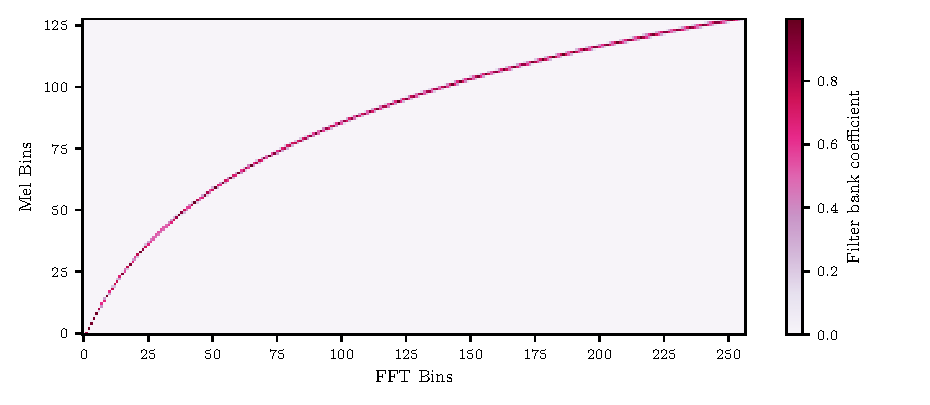
\includegraphics[width=1.0\linewidth]{img/plots/mel_filter_bank_matrix.pdf}
    \caption{Mel filter bank matrix ${H}$ in the case of $f_s=16\text{kHz}$, $M=128$ and $W_{\text{pad}}=512$.}
    \label{fig:mel-filter-matrix}
\end{figure}

\subsubsection{Application of the Filter Banks}
Finally, the obtained Filterbanks ${H}$ are applied to ${P}$ and the logarithm is computed:
\begin{equation}
{X} = \log_e({H} {P} + \epsilon) \in \mathbb{R}^{M \times L}
\end{equation}
where $\epsilon$ is a small constant to avoid logarithm of zero.

This results in ${X}$, the Mel spectrogram, where $M$ is the number of Mel bins and $L$ is the number of frames. Each frame of the Mel spectrogram is denoted as ${X}[i]$, for $i = 0, 1, \ldots, L-1$.

\subsection{Datasets}

For the pretraining task, we use AudioSet-2M \cite{gemmeke2017audio} and Librispeech \cite{panayotov2015librispeech}, enabling comparison with the results reported in \cite{gong2022ssast} and thus facilitating validation of our experimental setup and codebase. Combined, these two datasets consist of 5,734 hours of audio. 

For fine-tuning on \gls{sv}, in addition to the Librispeech dataset the VoxCeleb dataset \cite{nagrani2017voxceleb} is used. It comprises a diverse collection of speakers recorded in various settings, providing a rich landscape for assessing \gls{sv} efficacy. Combined, these two datasets consist of 3,368 hours of audio from 9,593 distinct speakers.

All audio files are converted to $f_s=16$kHz mono channel audio signals of 10 seconds, i.e. one-dimensional arrays of $l=160{,}000$ values. If the original audio file is longer than that, it is split into pieces. For audio files shorter than 10s, they are combined with other files.

As a preprocessing step, audio files are converted into mel spectrograms, using the procedure outlined in \ref{sec:mel_spectrogram_conversion}. Each spectrogram $X$ consists of $L$ frames with $M$ mel bins. A single frame covers a duration of 25 milliseconds ($\Rightarrow W=16\text{kHz}\cdot25\text{ms}=400$), and consecutive frames are shifted by 10 milliseconds ($\Rightarrow S=16\text{kHz}\cdot10\text{ms}=160$) relative to each other. The number of frames in a 10-second audio clip can be calculated using Equation \ref{eq:spectrogram_L}:
$$
L = \left\lfloor \frac{l - W}{S} + 1 \right\rfloor = \left\lfloor \frac{160000 - 400}{160} + 1 \right\rfloor = 998
$$
This calculates the total number of 25ms frames that can fit into 10 seconds, taking into account that each subsequent frame starts 10ms after the previous one. The number of Mel bins $M$ is set to 128 and a Hanning window is used. Consequently, the preprocessed data samples are all of size $998 \times 128$:
\[
    X =
    \begin{bmatrix}
    \vert & \vert & \vert & \vert & \vert &       & \vert  \\
    X[0]  & X[1]  & X[2]  & X[3]  & X[4]  &\cdots & X[997] \\
    \vert & \vert & \vert & \vert & \vert &       & \vert
    \end{bmatrix}
    \in \mathbb{R}^{128 \times 998}
\]


\section{Pretraining}
\label{methods_pretraining}

In this section, we describe the self-supervised pretraining algorithm developed by \cite{gong2022ssast}. As opposed to frameworks that either used a discriminative (e.g., wav2vec \cite{schneider2019wav2vec}) or a generative (e.g., APC \cite{chung2020generative}) loss function, the \gls{ssast} architecure employs a joint discriminative and generative objective for pretraining, which is summarized in Algorithm~\ref{alg:pretrain}.

\begin{algorithm}[h]
\caption{Joint Discriminative and Generative Masked Spectrogram Patch Modeling}
\label{alg:pretrain}
\begin{algorithmic}[1]
\Require{Unlabeled Audio Dataset $\mathcal{D}$, SSAST Model $\mathcal{M}$, Number of Masked Patches $N$}
\For{every epoch}
    \For{$X \in \mathcal{D}$}
        \State split $X$ into $T$ patches $x=\{x_0, x_1, ..., x_{T-1}\}$
        \State $E=\mathcal{M}_{\texttt{patch\_embedding}}(x)$ 
        \State $I=\text{RandomSample}(\{0, 1, \dots, T-1\}, N)$ \Comment{Select $N$ unique indices}
        \State $E_I$ = $E_{\texttt{mask}}$ \Comment{Mask the Patch Embeddings}
        \State $O=\mathcal{M}_{\texttt{Transformer}}(E+P)$
        \State $\mathcal{L}_d=0,\mathcal{L}_g=0$
        \For{$i\in I$}
            \State $r_i=\mathcal{M}_{\texttt{reconstruction\_head}}(O_i)$
            \State $c_i=\mathcal{M}_{\texttt{classification\_head}}(O_i)$
            \State $\mathcal{L} \mathrel{+}= \mathcal{L}_d(x_i,c_i,x_I) + \lambda\mathcal{L}_g(x_i,r_i)$
        \EndFor
        \State$\mathcal{L} = \mathcal{L}\mathbin{/}N$
        \State update $\mathcal{M}$ to minimize $\mathcal{L}$ 
    \EndFor
\EndFor 
\Return $\mathcal{M}$
\end{algorithmic}
\end{algorithm}

As mentioned above, the spectrograms $X$ are of size $998\times128$. They are then split into $T=L/2=499$ patches $x=\{x_0, x_1, ..., x_{498}\}$ of size $2 \times 128$ (2 frames in the time dimension with 128 mel frequency bins). These \textit{frame-like} patches $x$ henceforth serve as the basic processing unit of the model, similar to the subword tokens in an \gls{llm}:
\[
\underbrace{\begin{array}{cc}
\vert & \vert \\
X[0] & X[1] \\
\vert & \vert
\end{array}}_{x_0}
\underbrace{\begin{array}{cc}
\vert & \vert \\
X[2] & X[3] \\
\vert & \vert
\end{array}}_{x_1}
\cdots
\underbrace{\begin{array}{cc}
\vert & \vert \\
X[996] & X[997] \\
\vert & \vert
\end{array}}_{x_{498}}
\]

Each patch $x_i$ is converted to a corresponding 768-dimensional patch embedding $E_i$ using a linear projection layer, which is called \texttt{patch\_embedding}-layer. Then a set of indices $I$ is generated by randomly sampling $N$ unique numbers from $\{0, 1, ..., 498\}$. For each patch $x_i$ with an index $i \in I$, its patch embedding is replaced with a learnable mask embedding $E_{\texttt{mask}}$. Then, positional embeddings $P$ (also learnable) are added to the patch embeddings $E$ and the result is input to the (encoder-only) Transformer. Thus, the Transformer output $O$ ($499\times768$) is obtained. For each of the masked patches $x_i$, its corresponding $O_i$ is input to a classification head and a reconstruction head to get an output $c_i$ and $r_i$, respectively. 

The Transformer has an embedding dimension of 768, 12 layers, and 12 heads. Both the classification and reconstruction heads are two-layer \glspl{mlp} that map $O_i$ (768) to the same dimension as the (flattened) input patch $x_i$ (256). $r_i$ is expected to be close to $x_i$, and the model should learn to match correct ($x_i, c_i$) pairs. Therefore, the \gls{mse} loss $\mathcal{L}_g$ is used for the generative objective and the \gls{infonce} loss~\cite{oord2018representation} $\mathcal{L}_d$ for the discriminative objective:
\begin{equation}
\label{eq:MSE}
\mathcal{L}_g=\frac{1}{N}\sum_{i \in I} \text{mean}\left((r_i-x_i)^2\right)
\end{equation}
\begin{equation}
\label{eq:InfoNCE}
\mathcal{L}_d=\frac{-1}{N}\sum_{i \in I}\log_e\left(\frac{\exp(c_i * x_i)}{\sum_{j \in I}\exp(c_i * x_j)}\right)
\end{equation}
where $N$ is the number of masked patches and $*$ denotes the dot product. $\mathcal{L}_d$ and $\mathcal{L}_g$ are then added with a weight $\lambda$:
\begin{equation}
\label{eq:pretraining-loss}
\mathcal{L}=\mathcal{L}_d + \lambda\mathcal{L}_g
\end{equation}
Akin to \cite{gong2022ssast}, we set $\lambda=10$. Finally, the parameters are updated to minimize $\mathcal{L}$ using the \gls{adam} optimizer \cite{kingma2015adam}. 

The authors of \cite{gong2022ssast} found out that frame-based \gls{ssast} results in superior performance compared to patch-based \gls{ssast} for speech-related downstream tasks. Furthermore, they also found that masking $N=400$ of the $T=512$ frame-like patches surpasses masking $N=250$ patches. Consequently, we adopt this masking approach during pretraining, masking $N=390$ of the $T=499$ frame-like $2 \times 128$ patches for the pretraining, to obtain a similar ratio of number of masked patches $N$ / total number of patches $T$. During evaluation, we accidentily used $N=400$, making the task a bit harder during evaluation\footnote{Our code built on \cite{gong2022ssast}, and they always used $N=400$ for evaluation, independent of the number of masked patches used for training.}.

\glsunset{mo}%
\glsunset{ms}%
Two distinct pretraining instances are initiated using the \gls{ssast} architecture:
\vspace{-\parskip}
\begin{itemize}[topsep=0.5\parskip, itemsep=0.0\parskip, parsep=0.5\parskip]
    \item Pretraining on original spectrograms for 10 epochs (\gls{mo}).
    \item Pretraining on spectrograms with their frames shuffled randomly in time, disrupting the temporal structure (\gls{ms}). Since the losses quickly stabilize at the expected values (Algorithm \ref{alg:mse_shuffled} and Equation \ref{eq:expected_infonce}), 5 epochs are enough for this configuration.
\end{itemize}

This dual approach is designed to yield insights into the influence of the temporal spectrogram arrangement during pretraining on the model's learning process. While shuffling the frames eliminates the model's ability to leverage temporal features, the model can still make some predictions, such as assigning an equal probability to all masked patches in the classification task and predicting the average of the unmasked patches in the reconstruct head. 

We set the batch size to 48, which is twice as much as the original \gls{ssast}. We use an initial learning rate of $10^{-4}$, and cut it into half if the patch prediction accuracy on the validation set stops improving for 8k iterations. We pretrained the \gls{ssast} on 3 NVIDIA A100 GPUs, which took about 4.4 days in the case of the model trained on original spectrograms (\gls{mo}) and 2.2 days in the case of the model trained on shuffled spectrograms (\gls{ms}). 



\section{Finetuning}
\label{sec:met:finetuning}

\glsunset{moo}%
\glsunset{mos}%
\glsunset{mso}%
\glsunset{mss}%
Both models, \gls{mo} and \gls{ms}, having undergone pretraining as described in \ref{methods_pretraining}, are then finetuned for \gls{sv} on the VoxCeleb 1/2 and Librispeech dataset. The dataset for finetuning consists of 3368 hours of speaker utterances from 9593 different speakers. The fine-tuning protocol, including mean-pooling on the outputs of the transformer encoder followed by a linear layer to derive speaker embeddings, is executed as delineated in \cite{gong2022ssast}. Corresponding to the pretraining phase, fine-tuning is done on both the original ($\Rightarrow \mathcal{M}_\text{$\cdot$/o}$) and the shuffled ($\Rightarrow \mathcal{M}_\text{$\cdot$/s}$) spectrograms for each of the two pretraining conditions, which yields four distinct models, referred to as \gls{moo}, \gls{mos}, \gls{mso} and \gls{mss}.

To finetune the two pretrained models on the downstream task of \gls{sv} the main idea is to project the transformer embeddings into a new vector space where it is possible to differentiate between two speakers using a vector similarity metric \cite{chung2020ContrastiveLoss, chung2018voxceleb2}. The paper \cite{chung2018voxceleb2} showed a proof of concept for this strategy. It used the same dataset (VoxCeleb) for training and as the speaker embedding dimension 512 was chosen. 

This thesis investigates three different approaches to finetune the \gls{ssast} model; experiment 1 (\ref{methods_finetune_firstAttempt}), experiment 2 (\ref{methods_finetune_secondAttempt}) and experiment 3 (\ref{methods_finetune_thirdAttempt}).

\subsection{Experiment 1}
\label{methods_finetune_firstAttempt}
For the first experiment the same \gls{mlp} structure is used as suggested in the finetuning part in \cite{gong2022ssast}. It consists of a LayerNormalization and a fully connected layer with an input dimension of 768 and an output dimension of 527, which is very close to the approach described in \cite{chung2018voxceleb2}. As described above, both pretrained models are finetuned once on original spectrograms and once on shuffled spectograms. The performance of these four different models, \gls{moo}, \gls{mos}, \gls{mso} and \gls{mss}, is evaluated on original spectrograms and shuffled spectrograms using 100 different speakers from the dataset used for finetuning.

\subsection{Experiment 2}
\label{methods_finetune_secondAttempt}
In the second experiment, an \gls{mlp} is used with an output dimension of 256 and the same architecture as deployed in the classification head during the pretraining stage. The idea behind it is that the pretraining loss forces the classification head to create correct matches of masked patches and the corresponding embeddings. Therefore, this architecture should also have the potential to accurately generate inter- and intra-speaker embeddings. For performance evaluation 100 different speakers from the finetuning dataset have been used.

\subsection{Experiment 3}
\label{methods_finetune_thirdAttempt}
During evaluation and after consultations with our supervisor, Prof. Dr. Thilo Stadelmann, we have reasons to believe that the training time in Experiment~1 (Section \ref{methods_finetune_firstAttempt}) was not sufficient. Therefore a third experiment has been set up. It uses the same head as described in Experiment~1 (Section \ref{methods_finetune_firstAttempt}) because, as discussed in \ref{results_finetuning}, this head yields the most promising performance. This experiment has been run for 14 Epochs on the same dataset as described in \ref{sec:met:finetuning}. Unfortunatly, it was not possible for us to let the experiment run for more epochs due to time limitations. For performance evaluation 100 different speakers from the finetuning dataset have been used.

\subsection{Loss}
\label{methods_contrastive_loss}

For contrastive learning there are different loss functions that have been widely used in state-of-the-art \gls{sr} \cite{chung2020ContrastiveLoss, bjorn2019cosineloss}. The loss functions relevant for this thesis are discussed in the following subsections. 

The first approach was to use the triplet loss. This decision has been made because of the wide use of the triplet loss function in this domain. The downside of the triplet loss was that the implementation could not be made very efficient as we wanted it to be, because our code used a for-loop to iterate over the different output embeddings to calculate the loss. When using the cosine embedding loss, we were able to vectorize the loss calculation, which lead to faster training. The required time per sample for the triplet loss was 0.017 seconds on average. With the cosine embedding loss the time per sample decreased by almost 20\% to 0.014 seconds. 

To finalize our decision, we compared the performance of the two approaches by finetuning with both setup for one day. We have achieved similar results in terms of performance and therefore the more efficient implementation has been used. 


\subsubsection{Triplet Loss}
The triplet loss \cite{Schroff2015FaceNetAU} was our first approach. It is computed using the following equation:
% \begin{equation}
% \label{eq:triplet}
% \mathcal{L}(A, P, N)=\max \left(\|f(A)-f(P)\|_p-\|f(A)-f(N)\|_p+\alpha, 0\right)
% \end{equation}
\begin{equation}
\label{eq:triplet}
\mathcal{L}=\max \left(\|\mathcal{M}(X_A)-\mathcal{M}(X_P)\|_p-\|\mathcal{M}(X_A)-\mathcal{M}(X_N)\|_p+\alpha, 0\right)
\end{equation}
We set $p = 2$ and $\alpha = 1$, which is also the default for PyTorch \cite{paszke2019pytorch, PyTorchTripletMarginLoss}. In Equation \ref{eq:triplet}, $\mathcal{M}(X_A)$ denotes the output of the model (i.e. the speaker embedding) for the audio sample of an \textit{anchor} speaker, $\mathcal{M}(X_P)$ represents the embedding of an audio sample of the same speaker (a \textit{positive} sample) and $\mathcal{M}(X_N)$ is the embedding of a different speaker (a \textit{negative} sample). During the training process $\mathcal{M}(X_A)$ and $\mathcal{M}(X_P)$ are pulled closer to each other, while $\mathcal{M}(X_A)$ and $\mathcal{M}(X_N)$ are pulled apart, as illustrated in Figure \ref{fig:triplet_loss}.

\begin{figure}[h]
  \centering

  \begin{tikzpicture}[scale=1, every node/.style={font=\scriptsize}]
    % Define styles
    \tikzset{
      main node/.style={circle, draw, minimum size=0.4cm, inner sep=0},
      label node/.style={circle, minimum size=0.3cm}
    }

    % Define offset for right side nodes
    \newcommand{\offset}{10}


    % Left side

    % Place text node outside the circle
    \node[main node, fill=blue!30] (a) at (0,0) {};
    \node[above left=-0.15cm of a] {$\mathcal{M}(X_A)$};

    % Circles with margin label for left side
    \draw[thick] (a) circle (2.6cm);
    \draw[thick] (a) circle (1.5cm);
    \draw[thick, <->] (-2.6,0) -- node[above, fill=white] {\small$\alpha$} (-1.5,0);

    % Use polar coordinates for positioning nodes
    \node[main node, fill=red!30] (n) at (-45:1.5) {};
    \node[below=0.1cm of n.east, anchor=north] {$\mathcal{M}(X_N)$};
    \node[main node, fill=green!30] (p) at (30:3) {};
    \node[above=0.1cm of p.east] {$\mathcal{M}(X_P)$};
    \draw[thick, -Stealth] (a) -- (n);
    \draw[thick, -Stealth] (a) -- (p);


    % Right side

    % Place text node outside the circle
    \node[main node, fill=blue!30] (a2) at (\offset,0) {};
    \node[above left=-0.15cm of a2] {$\mathcal{M}(X_A)$};

    % Circles with margin label for right side
    \draw[thick] (a2) circle (2.6cm);
    \draw[thick] (a2) circle (1.5cm);
    \draw[thick, <->] (\offset - 2.6,0) -- node[above, fill=white] {\small$\alpha$} (\offset - 1.5,0);

    % Use polar coordinates for positioning nodes with offset
    \node[main node, fill=red!30] (n2) at ([shift={(\offset,0)}]-30:2.7) {};
    \node[below right=-0.2cm of n2] {$\mathcal{M}(X_N)$};
    \node[main node, fill=green!30] (p2) at ([shift={(\offset,0)}]45:1.4){};
    \node[above right=-0.2cm of p2.north east, anchor=south west] {$\mathcal{M}(X_P)$};
    \draw[thick, -Stealth] (a2) -- (n2);
    \draw[thick, -Stealth] (a2) -- (p2);


    % Training Arrow

    \path (a) -- (a2) node[midway, single arrow, draw=black, minimum width=20mm, minimum height=30mm, inner sep=0mm, single arrow head extend=3mm] {\normalsize Training};

  \end{tikzpicture}

  \caption{Visualization of the Triplet loss (adapted from \cite{matties2020vector}).}
  \label{fig:triplet_loss}
\end{figure}


\subsubsection{Cosine embedding loss}

The cosine embedding loss was the final loss function used for further evaluation. For two speakers with identity labels $a$ and $b$, it is computed using the following equation:
\begin{equation}
 \mathcal{L}= \begin{cases}1 - \operatorname{sim} \left(\mathcal{M}(X_a), \mathcal{M}(X_b)\right), & \text { if } a = b \\ \max \left(0, \operatorname{sim} \left(\mathcal{M}(X_a), \mathcal{M}(X_b)\right)-\alpha\right), & \text { if } a \neq b \end{cases},
\end{equation}
where $\mathcal{M}(X)$ is the output of the model for a Mel spectrogram $X$ and $\operatorname{sim}(\cdot, \cdot)$ denotes the cosine similarity of two vectors:
\begin{equation}
\operatorname{sim}(u, v) := \cos(\theta) = \frac{u * v}{\|u\| \|v\|}=\frac{\sum_{i=1}^n u_i v_i}{\sqrt{\sum_{i=1}^n u_i^2} \sqrt{\sum_{i=1}^n v_i^2}}.
\end{equation}
We set $\alpha=0$, which is also the default in Pytorch.




\subsection{Testing}

Each finetuned model is scrutinized under the same two testing conditions; on shuffled as well as on orinial spectrograms. This evaluation strategy is pivotal to discern whether models leverage temporal features. For performance evaluation, \gls{eer} and cosine similarity are calculated.

\subsubsection{\gls{eer} - Equal Error Rate}

\begin{figure}[htbp] % 'htbp' option is for placement of the figure
    \centering % This centers the figure in the column
        \begin{tikzpicture}
            
            % Improved labels for axes
            \draw[thick,->] (-0.5,0) -- (7.5,0) node[midway, below] {Threshold}; % Label x-axis, shifted downward for clarity
            \draw[thick,->] (0,-0.5) -- (0,4.5) node[midway, above, rotate=90] {Error Rate (\%)}; % Rotated y-axis label, shifted right for clarity

            % Hyperbola
            \draw[domain=0.5:7,variable=\x,smooth,thick] plot ({\x},{2/(\x/1.0)});
            \draw[domain=0.5:7,variable=\x,smooth,thick] plot ({\x},{2/(-((\x/1.0)-7.5))});
        
            % Labels
            \node at (7.5-1.2,3.5) [above] {FRR};
            \node at (1.2,3.5) [above] {FAR};
            
            % Make EER point and label red
            \node at (3.75,0.533) [circle,fill,inner sep=2pt, red]{}; % EER point in red
            \node at (3.75,0.65) [above, red] {EER}; % EER label in red
            
        \end{tikzpicture}
    \caption{Illustration of FAR and FRR curves with EER point.} % Caption for the figure
    \label{fig:eer_curve} % Label for referencing the figure
\end{figure}

The \gls{eer} is a popular benchmark in \gls{sv} for comparing model performance. It is well suited for the performance evaluation of binary classification models. It provides a single value that summarizes the system's performance by balancing two types of errors: false acceptances and false rejections. The \gls{eer} is defined as the point at which the \gls{far} and \gls{frr} are equal, as illustrated in Figure \ref{fig:eer_curve}.

\pagebreak [2]
Using the \gls{eer} as a performance metric makes it possible to conduct the \textsc{Neururer} examination \cite{neururer2023deep} as described in \ref{foundation_sst} and answer the main research question of this thesis.

\subsubsection{Cosine similarity}
In data analysis, cosine similarity is a measure of similarity between two non-zero vectors defined in an inner product space. Cosine similarity is the cosine of the angle between the vectors; that is, it is the dot product of the vectors divided by the product of their lengths. It follows that the cosine similarity does not depend on the magnitude of the vectors, but only on their angle \cite{HAN201239, Singhal2001ModernIR}.

Evaluating this metric can underline the statement beeing made by the \gls{eer} and directly verifies if the finetuned model has learned to differentiate between intra- and inter-speaker embeddings.

